\section{Modeling and Formal Methods: Concepts and Definitions}
\label{sec:concepts}
The contributions of this research require further information regarding specific concepts of formal methods. Our approach allows safety analysts to extend an existing system model with fault information. The nominal model can then be analyzed using formal methods of verification to show that in the absence of faults the system meets its specified requirements. The extended fault model can also be formally analyzed to show how active faults in the system may violate the specified properties. 

The existing system model is written in the Architecture Analysis and Design Language (AADL)~\cite{AADL_Standard}. This model is extended with behavioral contracts that formalize the requirements into temporal logic using the Assume-Guarantee Reasoning Environment (AGREE)~\cite{cofer2012compositional}. This constitutes the nominal system model. Verification through AGREE consists of a translation of the AADL model along with the AGREE contracts into a Lustre~\cite{Halbwachs91:IEEE} model. JKind~\cite{2017arXiv171201222G}, an infinite state model checker, is used to perform the formal verification of the Lustre model. Verification of the program is based on {\em k-induction} (see Section~\ref{sec:induction}) and property directed reachability using a back-end SMT solver such as Z3~\cite{z3} or SMTInterpol~\cite{smtInterpol}. 

Given this nominal model organization, we extend this to allow for reasoning about faults. This is detailed in Chapter~\ref{chap:faultModeling}. The remainder of this section includes concepts and definitions regarding the formalization of the nominal system model. 

\subsection{Architecture Analysis and Design Language}
The Architectural Analysis and Design Language (AADL) is an SAE International standard language that provides a unifying framework for describing the system architecture for performance-critical, embedded, real-time systems~\cite{AADL_Standard,FeilerModelBasedEngineering2012}. From its conception, AADL has been designed for the design and construction of avionics systems.  Rather than being merely descriptive, AADL models can be made specific enough to support system-level code generation.  
 
An AADL model describes a system in terms of a hierarchy of components and their interconnections, where each component can either represent a logical entity (e.g., application software functions, data) or a physical entity (e.g., buses, processors). An AADL model can be extended with language annexes to provide a richer set of modeling elements for various system design and analysis needs (e.g., performance-related characteristics, configuration settings, dynamic behaviors). The language definition is sufficiently rigorous to support formal analysis tools that allow for early phase error/fault detection. Further details regarding AADL will be introduced as needed throughout this dissertation. 

\subsection{Compositional Analysis in the Assume-Guarantee Reasoning Environment}
The {\em compositional} analysis of systems was introduced in order to address the scalability of model checking large software systems~\cite{pnueli1985transition, heckel1998compositional, NFM2012:CoGaMiWhLaLu}. {\em Monolithic} analysis flattens the hierarchical system model and use all model elements from all layers in order to find proof of a safety property. Compositional analysis, on the other hand, is performed per the architecture hierarchy such that analysis at a higher level is based on the components at the next lower level and conducted layer by layer; the components of a system are organized hierarchically and each layer of the architecture is viewed as a system. The idea is to partition the formal analysis of a system architecture into verification tasks that correspond into the decomposition of the architecture. 

A component contract in an assume-guarantee reasoning environment is an assume-guarantee pair. Intuitively, the meaning of a pair is: if the assumption is true, then the component will ensure that the guarantee is true. The formulation of assume-guarantee compositional reasoning  uses the past-time LTL\footnote{past-time LTL provides temporal operators that refer to the past states of an execution trace relative to a current point of reference} operators $G$ (globally), $U$ (until), $H$ (historically), and $Z$ (in the previous instant).

A component contract is an assume-guarantee pair $(A,P)$ for propositions $A, P$. Assume-guarantee reasoning attempts to prove that if the assumptions have held in all previous instances up to the current instance, then the guarantee holds at the current time~\cite{cofer2012compositional}; formally, this can be written as $G(H(A) \implies P)$. 

Each architectural layer is viewed as a system with inputs, outputs, and components. A system $S$ can be described as its own contract $(A_S, P_S)$ and the contracts of its components $C_S$. Thus, $S = (A_S, P_S, C_S)$. For each layer, the proof consists of demonstrating that the system guarantee is provable given the guarantees of its direct subcomponents and the system assumptions, or more formally prove $G(H(A_S) \implies P_S)$ given $G(H(A_C) \implies P_C)$ for each component $C$ in the system.  

Monolithic verification of an assume-guarantee reasoning environment attempts to prove the statement $G(H(A_S) \implies P_S)$ directly from the system and subcomponent assumptions. Compositional analysis, on the other hand, consists of $n+1$ verification tasks per layer for each n components. Component verification conditions establish that the assumptions of each component are implied by the system assumptions and the properties of sibling components. The $n^{th}+1$ task is the system level verification condition which shows that system guarantees follow from system assumptions and the properties of each subcomponent. This proof is performed one layer at a time starting from the top level of the system and composed accordingly.

When compared to monolithic analysis (i.e., analysis of the flattened model composed of all components), the compositional approach allows the analysis to scale to much larger systems~\cite{NFM2012:CoGaMiWhLaLu}. The {\em Assume-Guarantee Reasoning Environment} (AGREE)~\cite{cofer2012compositional} provides a way to perform compositional verification on models that are defined using the Architecture Analysis and Design Language (AADL)~\cite{aerospace2012sae}. More details on AGREE are given as needed throughout this document.

\subsection{Lustre}
\label{sec:lustre}
The AADL/AGREE model is translated into Lustre~\cite{Halbwachs91:IEEE}, a synchronous dataflow programming language that is suitable for the design of a critical system, specification of its critical properties, and verification of those properties. A Lustre variable or expression is considered to represent the sequence of values it takes during the whole execution of the program, and Lustre operators are considered to operate globally over these sequences~\cite{Halbwachs91:IEEE}. In other words, real time is abstracted into execution steps and the variables and expressions in the program take their values at each time step. 

\begin{figure}[h]
	\begin{center}
		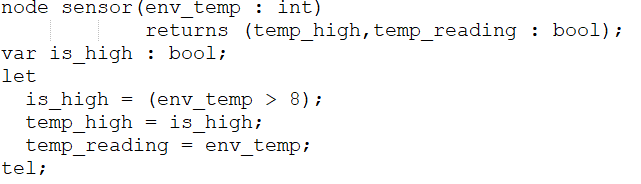
\includegraphics[width=0.6\textwidth]{images/lustreExample.PNG}
	\end{center}
	\caption{Sensor Node Defined in Lustre}
	\label{fig:lustreExample}
\end{figure}

A simple example of a sensor node is shown in Figure~\ref{fig:lustreExample}. There is a single input, \texttt{env\_temp}, and two outputs: \texttt{temp\_high} and \texttt{temp\_reading}. A local variable (\texttt{is\_high}) is defined and assignments are made in the \texttt{let} ... \texttt{tel;} body of the node. The input comes in and the sensor outputs a high indication and a reading of the environmental temperature. 

\subsection{JKind}
JKind is an open-source industrial infinite-state inductive model checker for safety properties~\cite{2017arXiv171201222G}. Models and properties in JKind are specified in Lustre~\cite{Halbwachs91:IEEE}, a synchronous dataflow language, using the theories of linear real and integer arithmetic. JKind uses SMT-solvers to prove and falsify multiple properties in parallel. To understand how this analysis proceeds, some formal definitions and descriptions must be provided. 

\subsection{State Machines and Transition Systems}
\label{subsec:trans}
A state machine (or state automaton) is a mathematical model of computation and consists of states, represented by nodes, and transitions between them, represented by directed edges. The change from one state to another is called a {\em transition}. The Lustre model is viewed as a state machine with transitions between these states defined through the properties of the nodes. 

Transition systems are directed graphs with nodes representing reachable states and edges representing transitions between them. In this research we consider \emph{safety properties} over infinite-state machines. The states are vectors of variables that define the values of state variables. We assume there are a set of legal \emph{initial states} and the safety property is specified as a formula over state variables. A \emph{reachable state space} means that all states are reachable from the initial state. 

Given a state space $U$, a transition system $(I,T)$ consists of an
initial state predicate $I : U \to \bool$ and a transition step
predicate $T : U \times U \to \bool$.
We define the notion of
reachability for $(I, T)$ as the smallest predicate $\reach : U \to
\bool$ which satisfies the following formulas:
\begin{gather*}
  \forall u.~ I(u) \Rightarrow \reach(u) \\
  \forall u, u'.~ \reach(u) \land T(u, u') \Rightarrow \reach(u')
\end{gather*}
A safety property $P : U \to \bool$ is a state predicate. A safety
property $P$ holds on a transition system $(I, T)$ if it holds on all
reachable states, i.e., $\forall u.~ \reach(u) \Rightarrow P(u)$,
written as $\reach \Rightarrow P$ for short. When this is the case, we
write $(I, T)\vdash P$.

\subsection{Induction}
\label{sec:induction}
For an arbitrary transition system $(I, T)$, computing reachability
can be very expensive or even impossible. Thus, we need a more
effective way of checking if a safety property $P$ is satisfied by the
system. The key idea is to over-approximate reachability. If we can
find an over-approximation that implies the property, then the
property must hold. Otherwise, the approximation needs to be refined.

A good first approximation for reachability is the property itself.
That is, we can check if the following formulas hold:
\begin{gather}
  \forall s.~ I(s) \Rightarrow P(s)
  \label{eq:ind-base} \\
  \forall s, s'.~ P(s) \land T(s, s') \Rightarrow P(s')
  \label{eq:ind-step}
\end{gather}
If both formulas hold then $P$ is {\em inductive} and holds over the
system. If (\ref{eq:ind-base}) fails to hold, then $P$ is violated
by an initial state of the system. If (\ref{eq:ind-step}) fails to
hold, then $P$ is too much of an over-approximation and needs to be
refined.

The JKind model checker~\cite{2017arXiv171201222G} used in this research uses {\em
  $k$-induction} which unrolls the property over $k$ steps of the
transition system. For example, 1-induction consists of formulas
(\ref{eq:ind-base}) and (\ref{eq:ind-step}) above, whereas
2-induction consists of the following formulas:
\begin{gather*}
\forall s.~ I(s) \Rightarrow P(s) \\
\forall s, s'.~ I(s) \land T(s, s') \Rightarrow P(s') \\
\forall s, s', s''.~ P(s) \land T(s, s') \land P(s') \land T(s',
  s'') \Rightarrow P(s'')
\end{gather*}
That is, there are two base step checks and one inductive step check.
In general, for an arbitrary $k$, $k$-induction consists of $k$
base step checks and one inductive step check as shown in
Figure~\ref{eq:k-induction} (the universal quantifiers on $s_i$ have
been elided for space). We say that a property is $k$-inductive if it
satisfies the $k$-induction constraints for the given value of $k$.
The hope is that the additional formulas in the antecedent of the
inductive step make it provable.

\begin{figure}[h!]
\begin{gather*}
I(s_0) \Rightarrow P(s_0) \\[-2pt]
%
\vdots \\[2pt]
%
I(s_0) \land T(s_0, s_1) \land \cdots \land T(s_{k-2}, s_{k-1})
\Rightarrow P(s_{k-1}) \\[2pt]
%
P(s_0) \land T(s_0, s_1) \land \cdots \land P(s_{k-1}) \land
T(s_{k-1}, s_k) \Rightarrow P(s_k)
\end{gather*}
\caption{$k$-induction formulas: $k$ base cases and one inductive
  step}
\label{eq:k-induction}
\end{figure}

In practice, inductive model checkers often use a combination of the
above techniques. Thus, a typical conclusion is of the form ``$P$ with
lemmas $L_1, \ldots, L_n$ is $k$-inductive''.

\subsubsection{The SAT Problem and SMT Solvers}
\label{sec:satsmt}
The Boolean Satisfiability (SAT) problem attempts to determine if there exists a total truth assignment to a given propositional formula, that evaluates to $true$. Generally, a propositional formula is any combination of the disjunction and conjunction of literals (as an example, $a$ and $\neg a$ are literals). For example, the proposition $a \land b$ is satisfiable; when $a$ and $b$ are assigned to $true$, the formula is satisfied, or true.  On the other hand, the proposition $a \land \neg a$ is unsatisfiable; no such assignment can be found to satisfy both $a$ and $\neg a$. 

Satisfiability Modulo Theories (SMT) solvers also address the SAT problem, but can work over propositional logic or predicate logic with quantifiers. An SMT solver works over a conjunction of literals, as is the case with SAT solvers, but the literals can be expressed as predicates over non-boolean variables, such as $x > 0$. A boolean literal can be satisfied with a finite number of possible assignments; this is not always the case with an SMT formula.


\textbf{UNSAT Cores and Minimal Unsatisfiable Subsets}
When analyzing a model, there are certain questions that may be asked about the model requirements. If a model is unsatisfiable with respect to some system level property, it is of benefit to know \emph{why} it is not satisfiable. 

A constraint system $C$ is an ordered set of $n$ abstract constraints $\{C_1, C_2, ..., C_n\}$ over a set of variables. The constraint $C_i$ restricts the allowed assignments of these variables in some way~\cite{liffiton2016fast}. Given a constraint system, we require some method of determining, for any subset $S \subseteq C$, whether $S$ is \textit{satisfiable} (SAT) or \textit{unsatisfiable} (UNSAT). Given a constraint system $C$, there are certain subsets of $C$ that are of interest in terms of satisfiability. Definitions 2-4 are taken from research by Liffiton et. al.~\cite{liffiton2016fast}. 

For a given unsatisfiable problem, SAT solvers (and SMT solvers) attempt to provide proof of unsatisfiability by providing a subset of UNSAT clauses known as \textit{UNSAT cores}. In general, this is useful information to have regarding the constraint system in question. 

\begin{definition} A Minimal Unsatisfiable Subset (MUS) $M$ of a finite constraint system $C$ is a subset $M \subseteq C$ such that $M$ is unsatisfiable and $\forall c \in M$ : $M \setminus \{c\}$ is satisfiable. 
\end{definition}

\begin{definition} UNSAT core: Let $C$ be a finite set of constraints and $U \subseteq C$ an unsatisfiable subset. A constraint $c \in U$ is an UNSAT core for $U$ if $U \setminus \{c\}$ is satisfiable. A set of all unsatisfiability cores of $U$ constitute an MUS for $C$. 
\end{definition}

Intuitively, an MUS is the minimal explanation of the constraint systems infeasability and the UNSAT cores are the building blocks of the MUS. In recent years, a number of efficient algorithms have been introduced to find MUSs~\cite{liffiton2005max} and most of them focus on finding a single such subset~\cite{belov2012towards, belov2013core, belov2012muser2}. More recently, algorithms have been introduced that can find all such minimal unsatisfiable subsets~\cite{GhassabaniGW16, Ghassabani2017EfficientGO,bendik2018online}. 


\textbf{Inductive Validity Cores} Given a complex model, it is useful to extract traceability information related to the proof; in other words, which elements of the model were necessary to construct the proof of a safety property. An algorithm was introduced by Ghassabani et al. to provide Inductive Validity Cores (IVC) as a way to determine which model elements are necessary for the inductive proofs of the safety properties for sequential systems~\cite{GhassabaniGW16}. Given a safety property of the system, a model checker is invoked to construct a proof of the property. The IVC generation algorithm extracts traceability information from the proof process and returns a minimal set of the model elements required in order to prove the property. Later research extended this algorithm in order to produce all minimal IVC elements (\aivcalg)~\cite{Ghassabani2017EfficientGO,bendik2018online}. 

The \aivcalg algorithm considers a constraint system consisting of the assumptions and contracts of system components and the negation of the safety property of interest (i.e. the top level event). It then collects all Minimal Unsatisfiable Subsets (MUSs) of this constraint system; these are the minimal explanations of the constraint systems infeasibility in terms of the \textit{negation} of the safety property. Equivalently, these are the minimal model elements necessary to prove the safety property. 

 

